\documentclass[11pt]{article}
\usepackage{geometry}                
\geometry{letterpaper}                   

\usepackage{graphicx}
\usepackage{amssymb}
\usepackage{epstopdf}
\usepackage{natbib}
\usepackage{amssymb, amsmath}
\DeclareGraphicsRule{.tif}{png}{.png}{`convert #1 `dirname #1`/`basename #1 .tif`.png}

%\title{Title}
%\author{Name 1, Name 2}
%\date{date} 

\begin{document}



\thispagestyle{empty}

\begin{center}

\includegraphics[width=5cm]{ETHlogo.eps}

\bigskip


\bigskip


\bigskip


\LARGE{ 	Lecture with Computer Exercises:\\ }
\LARGE{ Modelling and Simulating Social Systems with MATLAB\\}

\bigskip

\bigskip

\small{Project Report}\\

\bigskip

\bigskip

\bigskip

\bigskip


\begin{tabular}{|c|}
\hline
\\
\textbf{\LARGE{Insert Title Here}}\\
\textbf{\LARGE{...}}\\
\\
\hline
\end{tabular}
\bigskip

\bigskip

\bigskip

\LARGE{Name 1 \& Name 2}



\bigskip

\bigskip

\bigskip

\bigskip

\bigskip

\bigskip

\bigskip

\bigskip

Zurich\\
May 2008\\

\end{center}



\newpage

%%%%%%%%%%%%%%%%%%%%%%%%%%%%%%%%%%%%%%%%%%%%%%%%%

\newpage
\section*{Agreement for free-download}
\bigskip


\bigskip


\large We hereby agree to make our source code for this project freely available for download from the web pages of the SOMS chair. Furthermore, we assure that all source code is written by ourselves and is not violating any copyright restrictions.
Several external packages are used that are freely available at Matlab FileExchange under a BSU license. 
\begin{center}

\bigskip


\bigskip


\begin{tabular}{@{}p{3.3cm}@{}p{6cm}@{}@{}p{6cm}@{}}
\begin{minipage}{3cm}

\end{minipage}
&
\begin{minipage}{6cm}
\vspace{2mm} \large Fabio Crameri

 %\vspace{\baselineskip}

\end{minipage}
&
\begin{minipage}{6cm}

\vspace{2mm} \large Marcel Thielmann

\end{minipage}
\end{tabular}


\end{center}
\newpage

%%%%%%%%%%%%%%%%%%%%%%%%%%%%%%%%%%%%%%%



% IMPORTANT
% you MUST include the ETH declaration of originality here; it is available for download on the course website or at http://www.ethz.ch/faculty/exams/plagiarism/index_EN; it can be printed as pdf and should be filled out in handwriting


%%%%%%%%%% Table of content %%%%%%%%%%%%%%%%%

\tableofcontents

\newpage

%%%%%%%%%%%%%%%%%%%%%%%%%%%%%%%%%%%%%%%



\section{Abstract}

Hei M\"ase, we should first define what we mean by social and physical forces. I'm not sure if there is something like social forces between an agent and a wall. I mean normally there is not...

Hei F�bu, in dem Helbing paper gibts definitiv social forces zwischen Wand und den agents. Irgendwie soll das ausdr�cken, dass die agents nicht so nah an der Wand laufen wollen. Wir k�nnen aber auch argumentieren, dass diese Kr�fte in ner Paniksituation ziemlich wurscht sind.

I don't know how to make bold characters

\section{Individual contributions}
Marcel: 376 bugs
Fabio: 376 bugfixes


\section{Introduction and Motivations}

\section{Description of the Model}

\subsection{Social forces}
\subsubsection{Repulsive forces}

The "social" repulsive force defined here for the walls/buildings can be written in mathematical terms as

\begin{equation}
	{f_{iWS}} = \left\{ {{A_i}\exp \left[ {\frac{{\left( {{r_i} - {d_{iW}}} \right)}}{{{B_i}}}} \right]} \right\}{n_{iW}} ,
	\label{eq:fiWS}
\end{equation}

where $A_i$ and $B_i$ are constants, $n_{iW}$ is the normalized vector pointing from the pedestrian to the wall, $d_{iW}$ is the distance in between and $r_i$ is the size (i.e. radius) of the pedestrian (Helbing et al., 2000).

The physical wall forces can be divided into a normal force and a tangential force acting from the wall and written as

\begin{equation}
	{f_{iWPn}} = \left\{ {kg\left( {{r_i} - {d_{iW}}} \right)} \right\}{n_{iW}}
	\label{eq:fiWPn}
\end{equation}

and

\begin{equation}
	{f_{iWPt}} = \left\{ {\kappa g\left( {{r_i} - {d_{iW}}} \right)\left( {{v_i} \cdot {t_{iW}}} \right)} \right\}{t_{iW}} ,
	\label{eq:fiWPt}
\end{equation}

respectively. Here, the function $g$ is zero if the pedestrian does not touch the wall, $k$ and $\kappa$ are large constants and $(v_i \cdot t_{iW})$ is the tangential velocity difference.

The total repulsive force from the architecture can then be written as

\begin{equation}
	{f_{iW}} = {f_{iWS}} + {f_{iWPn}} - {f_{iWPt}} .
	\label{eq:fiW}
\end{equation}


\subsubsection{Attractive forces}
In our model, the sole attractive force is the exit force. As for the social forces, it is rather a psychological force representing the will of each agent to reach the exit. In this work, we chose value of the exit force to be proportional to the sum of the other psychological forces (in our code, one can choose a proportionality constant to adjust the exit force). To determine the direction of the exit force, we used two different approaches: i) the agent is drawn directly towards the exit, regardless of any obstacles in between him and an exit, and ii) the agent decides on its walking direction based on the estimate of the time it needs to reach the exit.\\
While i) is relatively straightforward to implement, there are several crucial drawbacks to this method: First, it does not reflect at all the decision process of a human agent, since obstacles between the agent and the exit are always taken into account. Second, 
\subsection{Physical forces}
\subsection{Walking speed}
\subsection{Flooding}

\section{Implementation}
This section is meant to both give an overview of the methods used in this code as well as to provide a documentation of the code. Therefore, some details are mentioned here that might not be crucial for any code that simulates pedestrian dynamics, but are needed in our implementation. 
\subsection{Initialization of Buildings and Agents}
\subsection{Social forces}

\subsubsection{Architecture forces}

Eq. \eqref{eq:fiWS} can be rewritten as

\begin{equation}
	{f_{iWS}} = \left\{ {{A_i}\left( {\exp \left[ {\frac{{ - {d_{iW}}}}{{{B_i}}}} \right] \cdot \exp \left[ {\frac{{{r_i}}}{{{B_i}}}} \right]} \right)} \right\}{n_{iW}}
	\label{eq:fiWS2}
\end{equation}



\subsubsection{Exit forces}
In this section, we show two approaches to tackle the problem of the psychological exit force. Using small and rather simple models, we show the differences that arise from the different implementations. We then choose one of

\subsubsection{Agent forces}
\subsection{Physical forces}

\subsubsection{Wall forces}

\subsubsection{Agent forces}
\subsection{Walking speed}
\subsection{Flooding}


\section{Simulation Results and Discussion}
\subsection{Simple evacuation bottleneck: One exit}
\subsubsection{direct exit force}

The simplest version of our code has one exit (Fig. \ref{fig:test1}). The attractive force on the agents is defined to be linear towards the exit, thereby neglecting obstacles in between. The agents will not move towards an opening in an obstacle but toward the exit itself. Moreover, this formulation inhibits the agents of running around a bigger obstacle. This is a strong simplification but suitable to test the code.
The behavior of the agents towards the repulsive walls and towards each other is satisfactory.

\begin{figure}
	\begin{center}
	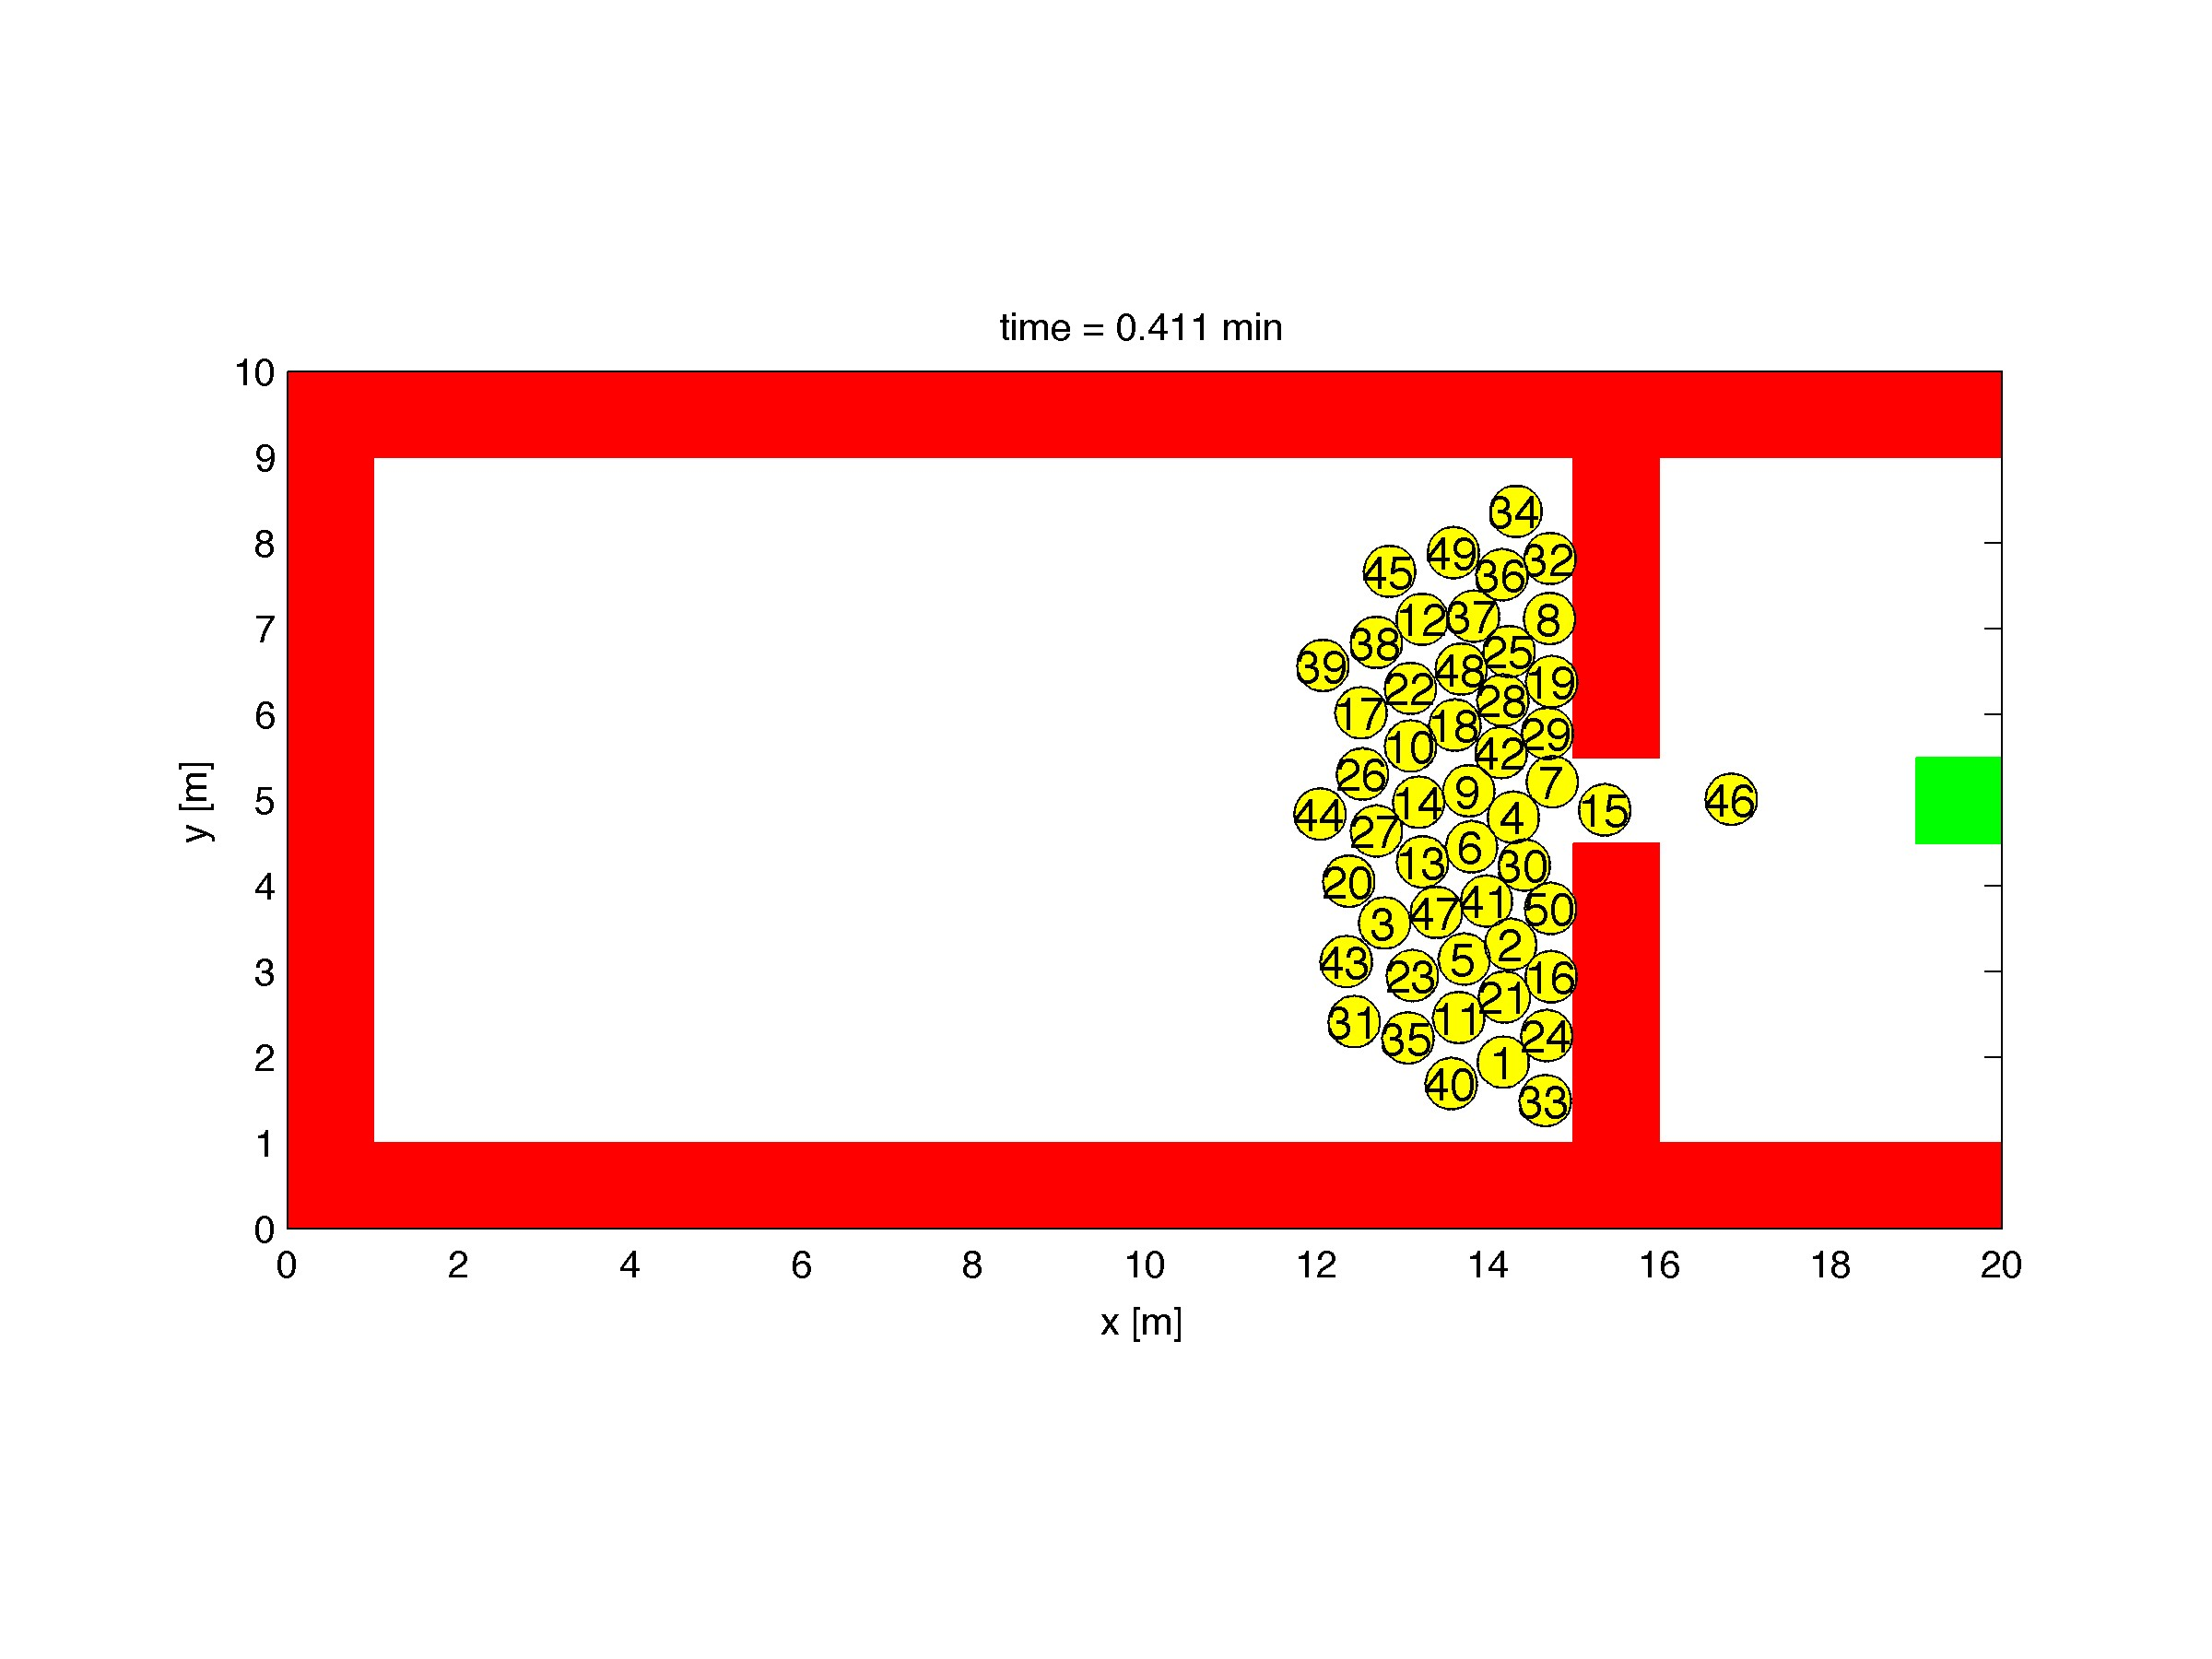
\includegraphics[width=16cm]{figures/test1000493.jpg}
	\caption{Simple simulation of an evacuation bottleneck. Agents (yellow) try to exit a room surrounded by repulsive walls (red) with an 1 m-wide door towards an attractive exit (green).}
	\label{fig:test1}
	\end{center}
\end{figure}

\subsubsection{shortest path formulation}
Finding the shortest path between two points is a mathematical problem that has received much attention since it's solution can be used in a huge number of applications. One of the earliest solutions to this problem was presented by Dykstra (reference). Shebian (right name? reference?) presented a fast and efficient method to solve a certain class of shortest path problems, which  is called the Fast marching method. It is a special case of level set methods and solve the Eikonal equation (equation?). This equation describes the We can essentially apply this algorithm to our problem
In a more sophisticated version of the code, we make use of a fast marching algorithm that takes into account walls as being regions with a low velocity. We compute the shortest path
subsection{Simple evacuation bottleneck: One exit with topography}
\subsection{Simple evacuation bottleneck: Two exits}
\subsection{Evacuation through a road network}
\subsection{Evacuation through a road network with topography and flooding}
\subsection{Evacuation of a beach in the case of a tsunami event}

\section{Summary and Outlook}

Christmas Tree!

\section{References}

- Helbing 2000




\end{document}  



 
